\documentclass[a4paper, 12pt, notitlepage]{report}

\usepackage{amsfonts} % if you want blackboard bold symbols e.g. for real numbers
\usepackage{graphicx} % if you want to include jpeg or pdf pictures
\setcounter{secnumdepth}{5}

\title{{\Huge Modelling Project} \vspace{300pt}} % change this
\author{Yoram Meijaard\\Chiel van Horssen\\Youri Haenen\\Bram Maas\\Martijn Ras\\Sascha Worms} % change this
\date{\today} % change this

\begin{document}

%%%%%%%%%% PRELIMINARY MATERIAL %%%%%%%%%%
\maketitle
\begin{center}
The report on the wheelchair problem of airline companies % change this
\\[12pt]
Supervised by: I. Papaliouras  % change this
\end{center}
\thispagestyle{empty}
\newpage
% \section*{Acknowledgement of Sources} % this must be included in undergradate projects
% For all ideas taken from other sources (books, articles, internet), the source of the ideas is mentioned in the main text and fully referenced at the end of the report.

% All material which is quoted essentially word-for-word from other sources is given in quotation marks and referenced.

% Pictures and diagrams copied from the internet or other sources are labelled with a reference to the web page or book, article etc.
% \\[12pt]
% Signed \dotfill Date \dotfill

\tableofcontents

%%%%%%%%%% MAIN TEXT STARTS HERE %%%%%%%%%%

%%%%%%%%%% SAMPLE CHAPTER %%%%%%%%%%
% \chapter{Summary}

% \chapter{Description of modeling process}

%first deadline
\chapter{Definition phase}
\section{Context}


\section{Problem definition and purpose}
\subsection{Model purpose}
\subsubsection{Three questions}
First things first, we have to answer three questions.:
Can you choose, does it output numbers and should your model produce value or knowledge.
Can you choose between solutions? Yes, there are different configurations for different sets of people, area and whatsoever belongs to the problem.
Does it output numbers? Yes, the model should produce a number of escort or wheelchairs to calculate the cost of the solution to the problem.
Does our model produce value or knowledge? Value, because it does not bring new knowledge, but it brings a more or less optimized solution to the problem.
Conclusion from this is: it is that the purpose of the model is a \textit{optimization}. It should produce the best possible solution for the owner.

\subsection{Model dimmensions}
\subsubsection{}
Now that we have figured out what our purpose, we have to figure out what the dimensions are:
\subsubsection{Continue or discrete}
First thing this is a discrete model, because all the input variables are whole numbers and the output number are also whole numbers. Most of our inbetween values are discrete numbers.
\subsubsection{Deterministic or stochastic}
We assume that this is deterministic, because the owner of the problem can decide on almost all the input. They have influence on how these values are delivered to the problem. Also we can assume that the amount of wheelchairs and disabled people follows pretty much in a deterministic pattern.
\subsubsection{Black box or glass box}
Glass box, because there is insight in what happens. It is all know by the owner.  The owner knows how many disabled people travel and where and when planes arrive and leave. Also they know the price for everything.
\subsubsection{Static or dynamic}
Static, time does not matter, because the model is just about one moment or one arrival time and one leaving time. All the input values are set before the model executes and they are valid through the entire model.
\subsubsection{Calculating or reasoning}
Calculating, because we eventually want to know a number. All the input values and quantities are known to be numbers.
\subsubsection{Geometrical or non-geometrical}
 Non-geometric, because we are not talking about a geometric setting, we do not define a airport as a geometrical figure. The only thing where we use distance is between gates and that is  allowed to be just an abstract number.
\subsubsection{Numerical or symbolic}
It is probably a little bit of both, because we start of using only symbols for the input eventually creating formulas, but the model will be used with concrete values for the input to be used to determine the output, which is going to be numerical.
\subsubsection{Material or immaterial}
Immaterial model, because there is no real airport modelled here. It is just a concept in our mind that we project into this immaterial model. It will sort of look like a modelling from scratch, the only difference is that we have a discrete model.

\subsection{Conceptual definition of the problem}
Given a description of the airport, incoming flights and outgoing flights: how many resources do we at least need to get all flights of the ground with all immobile people on board?

\section{Sub-questions}
\begin{enumerate}
\item How will the number of wheelchairs influence the amount of time of a transfer between two flights?
\item How will the location of the wheelchair depot influence the time?
	\begin{enumerate}
	\item What will this mean for the distance between the gates?
	\item What will this mean for the time required to travel between to gates?
	\item What will this mean for the maintenance of the wheelchairs
		\begin{enumerate}
		\item Who will do the maintenance of the wheelchairs?
		\item How much service does each wheelchair require?
		\item Where will those wheelchairs be bought?
		\end{enumerate}
	\item How will this influence the amount of escorts?
		\begin{enumerate}
		\item How many escorts do I need for one wheelchair?
		\end{enumerate}
	\item Will the storing of the chairs at one location decrease the costs of guarding them?
		\begin{enumerate}
		\item Will hiring additional security to guard the wheelchairs result in less damage/stolen chairs?
		\item If the escorts guard the chairs, how will this influence security?
			\begin{enumerate}
			\item Do we have to hire more escorts if they handle security?
			\end{enumerate}
		\end{enumerate}
	
	\end{enumerate}
\item What kind of wheelchairs will we take?
	\begin{enumerate}
	\item Will the quality of the chair influence the amount of maintenance required?
	\item Will the quality of the chair influence the amount of money we can ask for the service?
	\item How will the quality of the wheelchair influence the customer satisfaction?
		\begin{enumerate}
		\item How will this distinct us from other airliners?
		\item Will this create an increase in customers?
		\end{enumerate}
	\item Which wheelchair has the best price/quality rate?
		\begin{enumerate}
		\item How much is the difference in price?
			\begin{enumerate}
			\item How will the difference in price influence the total costs?
			\item What is the price of each wheelchair?
			\end{enumerate}
		\end{enumerate}
	\end{enumerate}
\item How will the amount of escorts influence the total costs?
	\begin{enumerate}
	\item What kind of people will escort the disabled?
		\begin{enumerate}
		\item Will the use of students influence the amount of customers that want to use the service?
		\item Will the use of athletes influence the average travel speed of an wheelchair?
		\item What kind of education/degree do they need?

		\end{enumerate}
	\item How much will we pay the escorts?
		\begin{enumerate}
		\item Will the salary of the escorts influence how hard they run?
		\item Will a  bonus for fast deliveries increase the efficiency?
			\begin{enumerate}
			\item Will this endanger the passengers?
			\end{enumerate}
		\end{enumerate}
	\item Will the use of electric wheelchairs decrease the amount the escorts?
		\begin{enumerate}
			\item Can everyone use an electric wheelchair?
		\end{enumerate}
	\end{enumerate}
		
\item How does the distance between gates influence the cost of transfer flights?
\item How does the walking speed of escorts influence the cost of transfer flights?
\item How does the cost depend on the time of travel between gates?
\end{enumerate}


\chapter{Conceptualization phase}
\section{Concepts, properties,values and relations}

\subsection{The model}
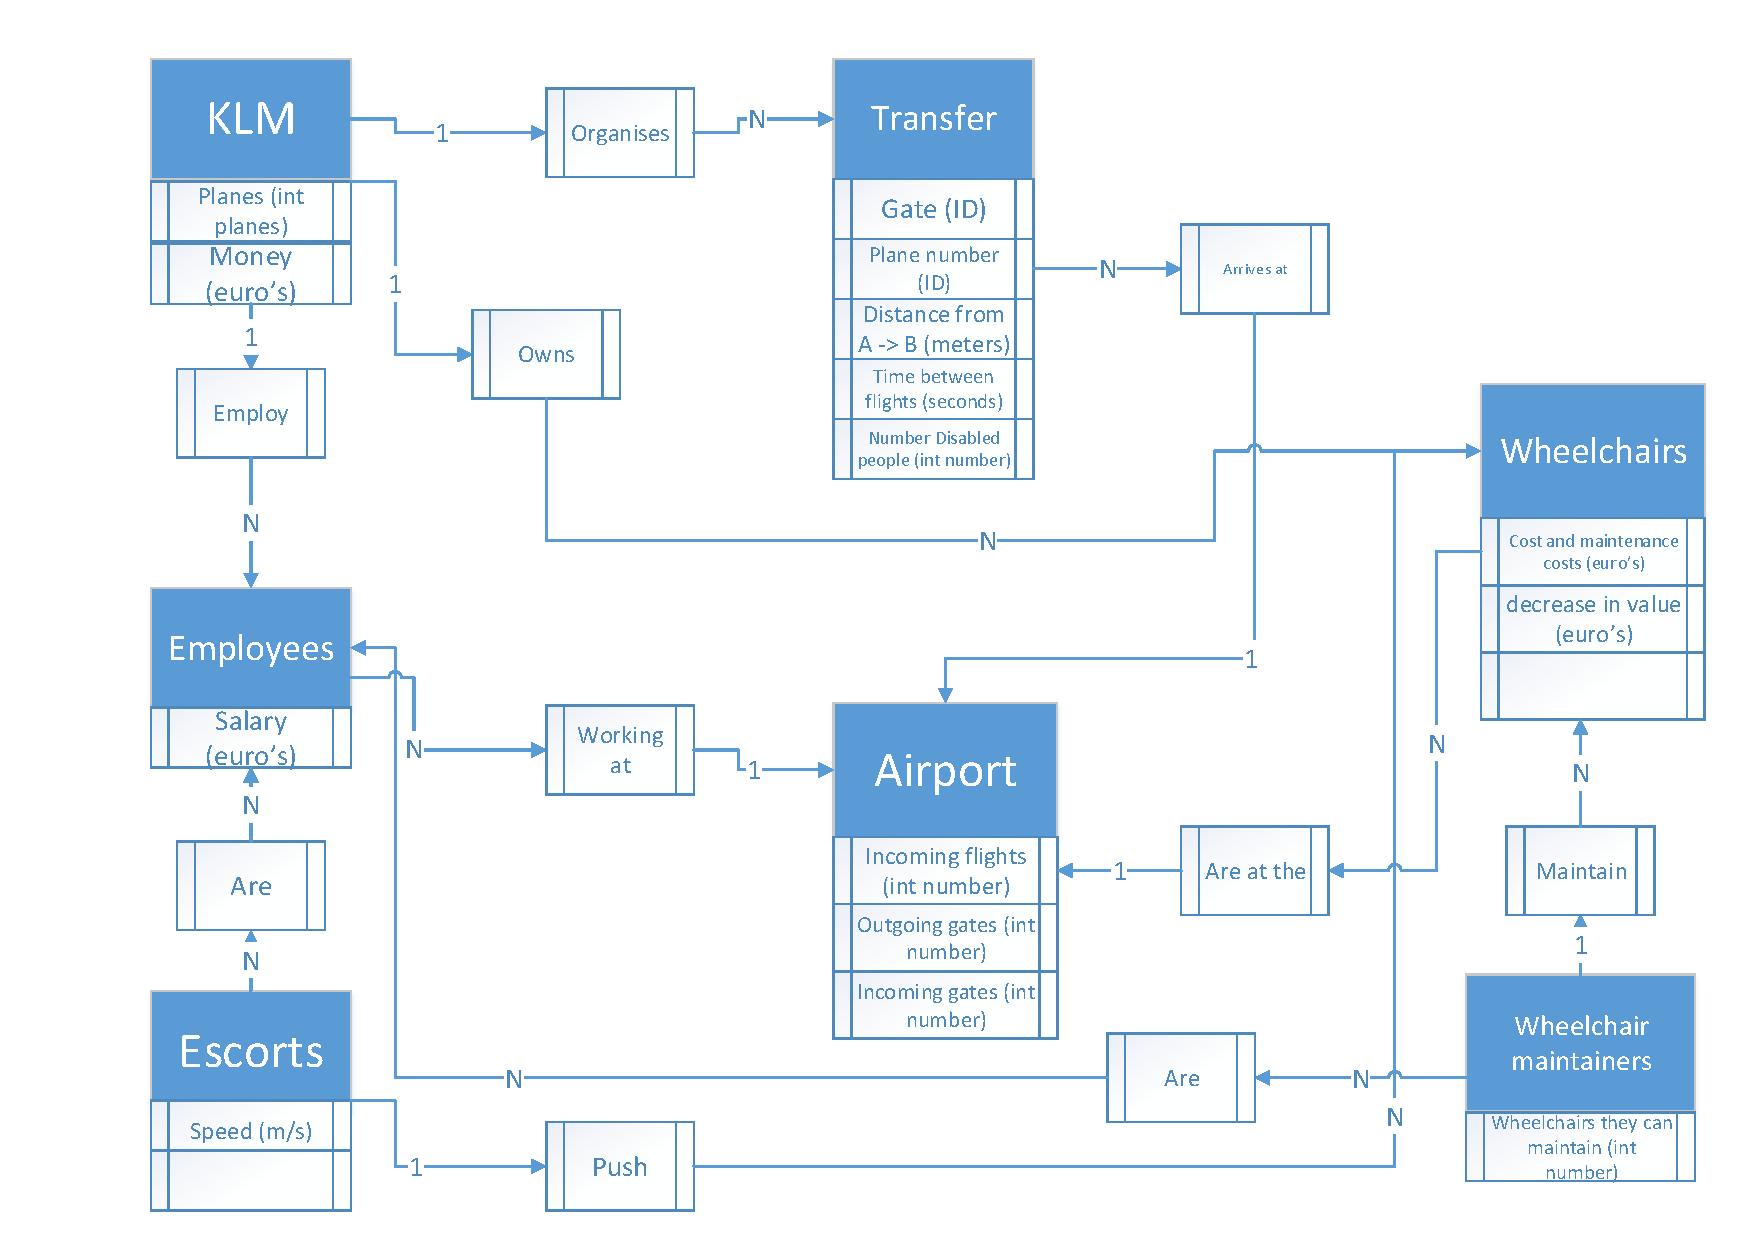
\includegraphics[scale=0.5]{Conceptualmodel.pdf}

\subsection{Explanation of}
\subsubsection{KLM}
The "Money" property is the amount of money KLM has in this model. 

\subsubsection{N on N relations of employees, escorts and maintainers}
These are very loose relations. In words this whould be: some employees are escorts and some employees are maintainers. 

\subsubsection{Time}
There two values that are described in the unit "euro's/time". This time is not a predetermined value, because we do not yet know in what timeframe we whould like to pay them. 

\subsubsection{Money}
As one can see, all of the quantities are eigher usable to determine the eventual amount of money or are already quantified in money.

%second deadline:
\chapter{Formalization phase}
\section{Quantities and their relationships}

\subsection{KLM}
\begin{description}
\item[Property:] Money
\item[Unit:] Euro's
\item[Role:] 
\end{description}
\subsection{Employees}
\begin{description}
\item[Property:] Salary
\item[Unit:] Euro's / hour
\item[Role:]
\end{description}
\subsection{Transfer} 
\begin{description}
\item[Property:] Distance from gate A to B
\item[Unit:] Meters
\item[Role:] 
\end{description}
\begin{description}
\item[Property:] Time between flights
\item[Unit:] Seconds
\item[Role:] To be chosen
\end{description}
\begin{description}
\item[Property:] Disabled people
\item[Unit:] An integer number
\item[Role:] To be chosen
\end{description}
\subsection{Escorts}
\subsection{Wheelchairs}
\subsection{Wheelchair maintainers}

\section{Approximations and assumptions}
\section{Derivations}
\section{Special cases}
\section{Estimates}

\chapter{Execution phase}
\section{Rephrased problem in formal terms}

%third deadline
% \section{Calculation, implementation and simulation}
% \section{Validation and verification; accuracy and precision}

% \chapter{Conclusion phase}
% \section{Presentation and interpretation}

% \chapter{Reflection and discussion}
% \section{Discussion after the conceptual model}
% \section{Discussion after the formal model}
% \section{Discussion after the result}
% \section{Discussion after the solution of the initial problem}

%%%%%%%%% INFORMATION %%%%%%%%%%
% \section{A Note About References}

% The Third and Fourth Year Handbook, and the Third and Fourth Year Project Handbook, have some clear guidelines about plagiarism and referencing.
% You should consult your project supervisor about the correct format for handling references.

% This document uses the `in-text' or Harvard system of referencing, which is a good default format.
% This requires both in-text citations and a list of references at the end of the document.
% The project templates have an example of a list of references.

% Within the text you must cite the authors surname(s) and the date of publication.
% When referring to a specific idea, or a direct quote, you must also give the page number.
% If there are two authors, use `and' and if there are more, use `et al.'\ and give all the authors names at the end.

% There are two styles of citation, implicit and explicit.
% Both are equally acceptable and it is also acceptable to mix and match.

% \subsubsection{Examples of implicit in-text citations}

% The sum of convex functions is itself convex (Blacke, 1985) and therefore any minimiser of this objective function will be a global minimiser (Greene and Whit, 1995, p.123). It is possible to exploit this fact (Browne et al., 2005) to enhance the optimisation algorithm.

% \subsubsection{Examples of explicit in-text citations}

% Blacke (1985) first proved that a sum of convex functions is convex. Any minimiser of this objective function will be a global minimiser, a fact shown by Greene and Whit (1995, p.123) and exploited by Browne et al.\ (2005) to enhance the optimisation algorithm.

%%%%%%%%% APPENDIX %%%%%%%%%%
% \appendix
% \chapter{An Appendix may not be necessary}

% Text introducing the/this appendix.

% \section{Appendix section}

% Text of this section.

% subsubsections and further divisions can also be used in appendices.

%%%%%%%%% BIBLIOGRAPHY %%%%%%%%%%
% \chapter*{Bibliography}

% \begin{description}

% \item Author, I. (Year). \emph{Book Title}, Publisher; Place of publication.

% \item Lamport, L. (1986), \emph{\LaTeX: A Document Preparation System}, Addison-Wesley; Reading, MA.

% \item Author, I. (Year). `Journal article title', \emph{Journal}, \textbf{Vol}, pp.first--last.

% \item Smith, A.D.A.C. and Wand, M.P. (2008). `Streamlined variance calculations for semiparametric
% mixed models', \emph{Statistics in Medicine}, \textbf{27}, pp.435--48.

% \end{description}

\end{document}
